\documentclass[12pt,a4paper]{article}
 
\usepackage{float}
%für feststellen der figures und tables [H] dranschreiben
\usepackage{units}
%wird so benutzt: 
%\unit[value/Zahl]{dimension/Einheit} oder 
%\unitfrac[value/Zahl]{dimension/Einheit num/Zähler}{dimension/Einheit denum/Nenner} oder
%\nicefrac[fontcommand/Schriftart]{dimension/Einheit num/Zähler}{dimension/Einheit denum/Nenner}

\usepackage{caption}
\usepackage{subcaption}

\usepackage[left=2cm,right=2cm,top=2cm,bottom=2cm]{geometry}
\usepackage[utf8]{inputenc}
\usepackage[T1]{fontenc}
\usepackage{lmodern}
\usepackage[ngerman]{babel}
\usepackage{amsmath}
\usepackage{graphicx}
 
%niemals zwei überschriften direkt übereinander schreiben, also immer mindestens in einem satz was sinnvolles unter jede überschrift schreiben (bei den versuchen z.B. das versuchsziel) 
\begin{document}
%deckblatt erstellen.


\begin{titlepage}

\begin{center}
% Oberer Teil der Titelseite:

\includegraphics[width=0.75\textwidth]{logo.pdf}\\[1cm]    	%Logo 

\textsc{\LARGE Bergische Universität Wuppertal}\\[1.5cm]	%Institution

\textsc{\Large Elektronik Praktikum}\\[0.5cm]				%Projekt


\newcommand{\HRule}{\rule{\linewidth}{0.5mm}}
\HRule \\[0.4cm]
{ \huge \bfseries Versuch EP10 Digitalelektronik
Teil 3: Mikrocontroller}\\[0.4cm]				%Titel

\HRule \\[1.5cm]

% Author und Tutor
\begin{minipage}{0.4\textwidth}
\begin{flushleft} \large
\emph{Autoren:}\\
Henrik \textsc{Jürgens} \\
Frederik \textsc{Strothmann}
\end{flushleft}
\end{minipage}
\hfill
\begin{minipage}{0.4\textwidth}
\begin{flushright} \large
\emph{Tutoren:} \\
Hans-Peter \textsc{Kind} \\
Peter \textsc{Knieling} \\
Marius \textsc{Wensing}
\end{flushright}
\end{minipage}

\vfill

% Unterer Teil der Seite/Datum
{\large \today}

\end{center}

\end{titlepage}

\newpage
\tableofcontents
\newpage
\section{Einleitung}
%einleitung zu dem experiment.
%auf die einstellungen, die vor dem versuch gemacht werden, eingehen oder auf eine anleitung dazu verweisen
%es soll immer erwähnt werden um was es in dem Versuch geht und wie das relisiert werden soll
%---------------------------------------------------------------------------------------------
%hinter der einleitung kann der allgemeine theoretische hintergrund in einer zusätzlichen section erklärt werden
%1-----------------------------------------------1
In diesem Versuch geht es um Mikrocontroller und deren Programmierung. Es werden das ansteuern von LEDs, das verwenden von Tastern, die Verwendung eines Oszillators und die Verwendung des ACDs behandelt. Als Versuchsboard wird das Board in Abbildung \ref{fig:board} verwendet.

%In diesem Versuch soll zu jedem Arbeitsschritt eine kurze Beobachtung dokumentiert werden, sowie auch der Quellcode selber, welcher möglichst gut kommentiert werden soll.

\begin{figure}[H] 
  \centering 	
    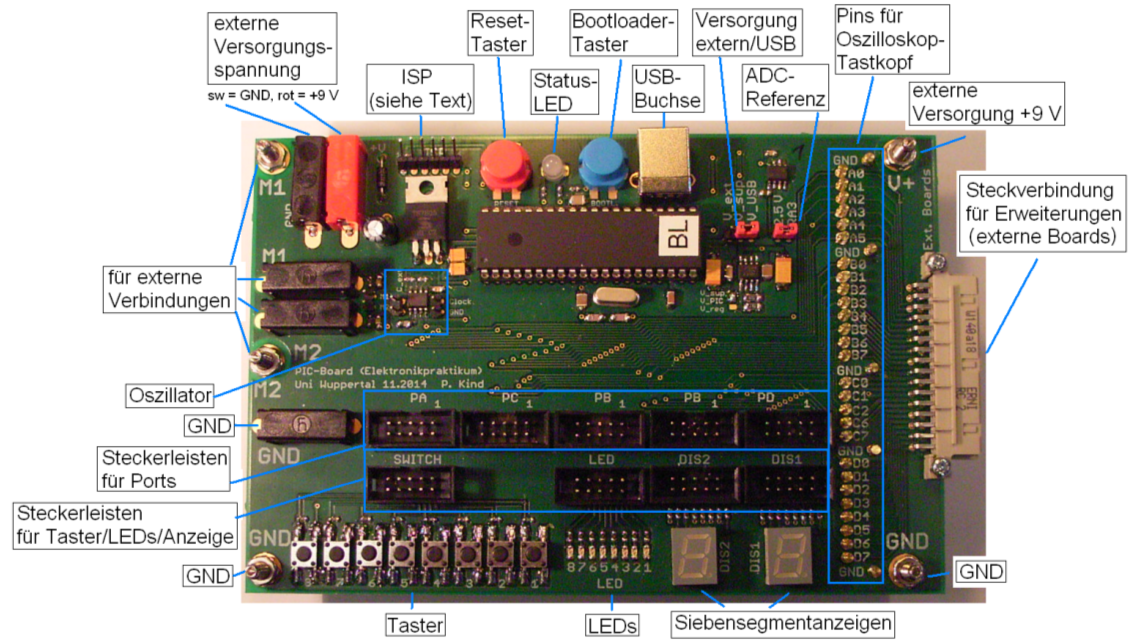
\includegraphics[ scale = 0.4]{board.png}
  	\caption[Versuchsboard]{Versuchsboard\footnotemark}
  \label{fig:board}
\end{figure}
\footnotetext{Abbildung entnommen von http://www.atlas.uni-wuppertal.de/$\sim$kind/ep10\_14.pdf am 10.01.2015}

\section{Messen der Arbeitsgeschwindigkeit des PIC18F4455}
%kurz das ziel dieses versuchsteiles ansprechen, damit keine zwei überschriften direkt übereinander stehen!
%bei schwierigeren versuchen kann auch der theoretische hintergrund erläutert werden. (mit formeln, herleitungen und erklärungen)

In diesem Versuchsabschnitt wird die Arbeitsgeschwindigkeit des Mikrcontrollers untersucht, dafür wird eine LED mit schiedenen Schleifen und delay-Befehlen an und aus geschaltet.

\subsection{Schnellstmögliches Programm, ohne Verzögerungsbefehle}
%kurz das ziel dieses versuchsteiles ansprechen, damit keine zwei überschriften direkt übereinander stehen!
%bei schwierigeren versuchen kann auch der theoretische hintergrund erläutert werden. (mit formeln, herleitungen und erklärungen)

In diesem Versuchsteil wird eine LED abwechselt der Zustand 'AN' und 'AUS' zugewiesen. Dies geschied mit einer 'while(1)' Schleife.

\subsubsection*{Verwendete Geräte}
%(immer) eine skizze oder ein foto einfügen, die geräte/materialien !nummerieren! und z.b. eine legende dazu schreiben, besser wäre es das ganze in einem Fließtext gut zu beschreiben.
%falls am anfang des versuches nicht klar ist, was alles verwendet wird, wenn möglich erst am ende ein großes foto von den verwendeten materialien machen!\\

Es wird ein Netzgerät, ein PC, ein Verbindungskabel, ein Oszillsokop und das Versuchsboard verwendet.

\subsubsection*{Versuchsaufbau}
%skizze zum versuchsaufbau (oder foto) einfügen,   es muss erklärt werden wie das ganze funktioniert und welche speziellen einstellungen verwendet wurden (z.b. welche knöpfe an den geräten für die messung verdreht wurden)

In allen Versuchsteilen wird das Board in Abbilung \ref{fig:board_2} verwendet. Der Versuchsaufbau ändert sich im Folgendem nicht.

\begin{figure}[H] 
  \centering 	
    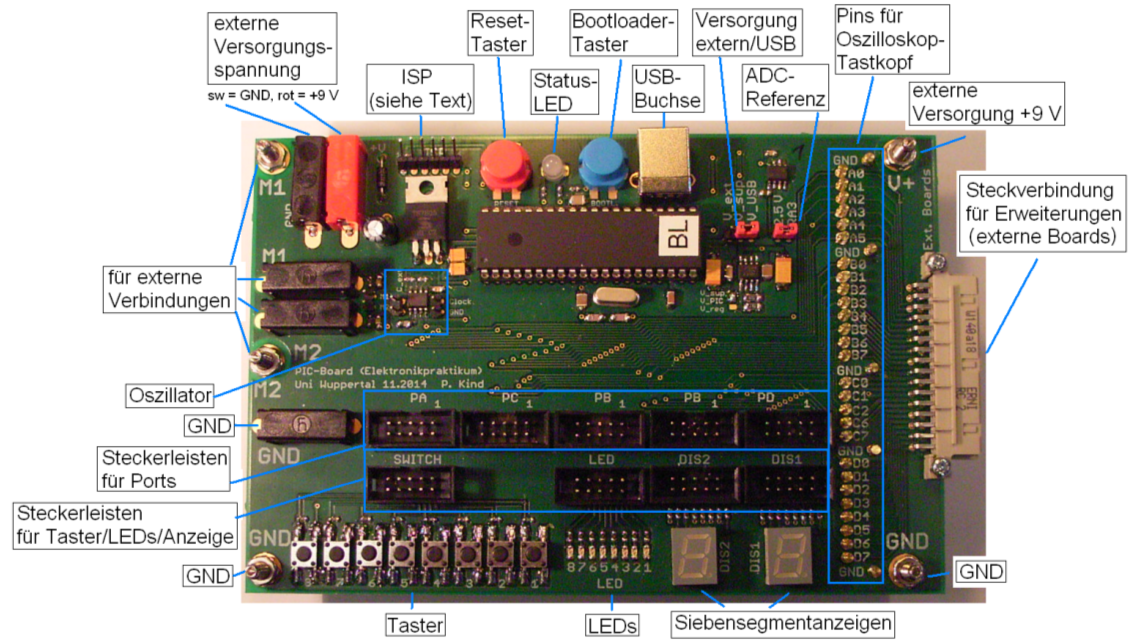
\includegraphics[ scale = 0.4]{board.png}
  	\caption[Versuchsboard]{Versuchsboard\footnotemark}
  \label{fig:board_2}
\end{figure}
\footnotetext{Abbildung entnommen von http://www.atlas.uni-wuppertal.de/$\sim$kind/ep10\_14.pdf am 10.01.2015}

\subsubsection*{Versuchsdurchführung}
%erklären, !was! wir machen, !warum! wir das machen und mit welchem ziel
%(wichtig) präzize erklären, wie bei dem versuch vorgegangen und was gemacht wurde

Es wird der Code ?? auf den Mikrokontroller geladen. Dann wird das Board an ein Oszilloskop angeschlossen und die Ausgangsfrequenz an den Pins gemessen.

\subsubsection*{Messergebnisse}
%die messwerte in !übersichtlichen! tabellen angegeben
%zu viele kleine tabellen in große tabellen überführen!
%zu große tabellen mit dem [scale]-befehl scalieren oder (falls zu lang) in zwei kleinere tabellen aufteilen
%(wichtig) vor !jeder! tabelle sagen, was gemessen wurde und wie die fehler gewählt wurden und ausreichend !erklären!, !warum! wir unsere fehler grade so gewählt haben
\subsubsection*{Auswertung}
%zuerst !alle! errechneten werte entweder in ganzen sätzen aufzählen, oder in tabellen (übersichtlicher) dargestellen, sowie auf die verwendeten formeln verweisen (die referenzierung der formel kann in der überschrift stehen)
%kurz erwähnen (vor der tabelle), warum wir das ganze ausrechnen bzw. was wir dort ausrechnen
%danach histogramme und plots erstellen, wobei wenn möglich funktionen durch die plots gelegt werden (zur not können auch splines benutzt werden, was aber angegeben werden muss)
%bei fits immer die funktion und das reduzierte chiquadrat mit angegeben, wobei auf verständlichkeit beim entziffern der zehnerpotenzen geachtet werden muss z.b. f(x)=(wert+-fehler)\cdot10^{irgendeine zahl}\cdot x + (wert+-fehler)\cdot10^{irgendeine zahl}
%bei jedem fit erklären, nach welchem zusammenhang gefittet wurde und warum!
%bei plots darauf achten, dass die achsenbeschriftung (auch die tics) die richtige größe haben und die legende im plot nicht die messwerte verdeckt
%kurz die aufgabenstellung abhandeln
%2-----------------------------------------------2
\subsection{Programm mit Verzögerungsbefehlen aus for-Schleifen}
%kurz das ziel dieses versuchsteiles ansprechen, damit keine zwei überschriften direkt übereinander stehen!
%bei schwierigeren versuchen kann auch der theoretische hintergrund erläutert werden. (mit formeln, herleitungen und erklärungen)

In diesem Versuchsteil soll wieder eine LED ein- und ausgeschaltet werden, jedoch mit einer verzögerung. Die Verzögerung soll mit hilfe einer for-schleife realisiert werden.

\subsubsection*{Verwendete Geräte}
%(immer) eine skizze oder ein foto einfügen, die geräte/materialien !nummerieren! und z.b. eine legende dazu schreiben, besser wäre es das ganze in einem Fließtext gut zu beschreiben.
%falls am anfang des versuches nicht klar ist, was alles verwendet wird, wenn möglich erst am ende ein großes foto von den verwendeten materialien machen!\\

Es wird ein Netzgerät, ein PC, ein Verbindungskabel, ein Oszillsokop und das Versuchsboard verwendet.

\subsubsection*{Versuchsdurchführung}
%erklären, !was! wir machen, !warum! wir das machen und mit welchem ziel
%(wichtig) präzize erklären, wie bei dem versuch vorgegangen und was gemacht wurde

Es wird der Code ?? auf den Mikrokontroller geladen. Dann wird das Board an ein Oszilloskop angeschlossen und die Ausgangsfrequenz an den Pins gemessen.

\subsubsection*{Messergebnisse}
%die messwerte in !übersichtlichen! tabellen angegeben
%zu viele kleine tabellen in große tabellen überführen!
%zu große tabellen mit dem [scale]-befehl scalieren oder (falls zu lang) in zwei kleinere tabellen aufteilen
%(wichtig) vor !jeder! tabelle sagen, was gemessen wurde und wie die fehler gewählt wurden und ausreichend !erklären!, !warum! wir unsere fehler grade so gewählt haben
\subsubsection*{Auswertung}
%zuerst !alle! errechneten werte entweder in ganzen sätzen aufzählen, oder in tabellen (übersichtlicher) dargestellen, sowie auf die verwendeten formeln verweisen (die referenzierung der formel kann in der überschrift stehen)
%kurz erwähnen (vor der tabelle), warum wir das ganze ausrechnen bzw. was wir dort ausrechnen
%danach histogramme und plots erstellen, wobei wenn möglich funktionen durch die plots gelegt werden (zur not können auch splines benutzt werden, was aber angegeben werden muss)
%bei fits immer die funktion und das reduzierte chiquadrat mit angegeben, wobei auf verständlichkeit beim entziffern der zehnerpotenzen geachtet werden muss z.b. f(x)=(wert+-fehler)\cdot10^{irgendeine zahl}\cdot x + (wert+-fehler)\cdot10^{irgendeine zahl}
%bei jedem fit erklären, nach welchem zusammenhang gefittet wurde und warum!
%bei plots darauf achten, dass die achsenbeschriftung (auch die tics) die richtige größe haben und die legende im plot nicht die messwerte verdeckt
%kurz die aufgabenstellung abhandeln
%2-----------------------------------------------2

\subsection{Programm mit Compiler-Verzögerungsbefehlen}

In diesem Versuchsteil soll eine Verzögerung des Ein- und Ausschaltvorgangs der LED mit Compiler-Verzögerungsbefehlen realisiert werden. Bei dieser Art der Verzögerung wird eine bestimmte Anzahl von Taktzyklen ausgesetzt.

\subsubsection*{Verwendete Geräte}

Es wird ein Netzgerät, ein PC, ein Verbindungskabel, ein Oszillsokop und das Versuchsboard verwendet.

\subsubsection*{Versuchsdurchführung}

Es wird der Code ?? auf den Mikrokontroller geladen. Dann wird das Board an ein Oszilloskop angeschlossen und die Ausgangsfrequenz an den Pins gemessen.

\subsubsection*{Messergebnisse}

\subsubsection*{Auswertung}

\subsubsection*{Diskussion}

\subsection{Programm mit fertigen Verzögerungsbefehlen}
%kurz das ziel dieses versuchsteiles ansprechen, damit keine zwei überschriften direkt übereinander stehen!
%bei schwierigeren versuchen kann auch der theoretische hintergrund erläutert werden. (mit formeln, herleitungen und erklärungen)

In diesem Versuchsteil soll das An- und Ausschalten der LED mit den verschiedenen Verzögerungsbefehlen realisiert werden. Verzögerungsbefehle sorgen für eine Verzögerung von einer bestimmten Zeitspannne und nicht wie Vorher für ein Aussetzen einer Anzahl von Taktzyklen.

\subsubsection*{Verwendete Geräte}
%(immer) eine skizze oder ein foto einfügen, die geräte/materialien !nummerieren! und z.b. eine legende dazu schreiben, besser wäre es das ganze in einem Fließtext gut zu beschreiben.
%falls am anfang des versuches nicht klar ist, was alles verwendet wird, wenn möglich erst am ende ein großes foto von den verwendeten materialien machen!\\

Es wird ein Netzgerät, ein PC, ein Verbindungskabel, ein Oszillsokop und das Versuchsboard verwendet.

\subsubsection*{Versuchsdurchführung}
%erklären, !was! wir machen, !warum! wir das machen und mit welchem ziel
%(wichtig) präzize erklären, wie bei dem versuch vorgegangen und was gemacht wurde

Es wird der Code ?? auf den Mikrokontroller geladen. Dann wird das Board an ein Oszilloskop angeschlossen und die Ausgangsfrequenz an den Pins gemessen.

\subsubsection*{Messergebnisse}
%die messwerte in !übersichtlichen! tabellen angegeben
%zu viele kleine tabellen in große tabellen überführen!
%zu große tabellen mit dem [scale]-befehl scalieren oder (falls zu lang) in zwei kleinere tabellen aufteilen
%(wichtig) vor !jeder! tabelle sagen, was gemessen wurde und wie die fehler gewählt wurden und ausreichend !erklären!, !warum! wir unsere fehler grade so gewählt haben
\subsubsection*{Auswertung}
%zuerst !alle! errechneten werte entweder in ganzen sätzen aufzählen, oder in tabellen (übersichtlicher) dargestellen, sowie auf die verwendeten formeln verweisen (die referenzierung der formel kann in der überschrift stehen)
%kurz erwähnen (vor der tabelle), warum wir das ganze ausrechnen bzw. was wir dort ausrechnen
%danach histogramme und plots erstellen, wobei wenn möglich funktionen durch die plots gelegt werden (zur not können auch splines benutzt werden, was aber angegeben werden muss)
%bei fits immer die funktion und das reduzierte chiquadrat mit angegeben, wobei auf verständlichkeit beim entziffern der zehnerpotenzen geachtet werden muss z.b. f(x)=(wert+-fehler)\cdot10^{irgendeine zahl}\cdot x + (wert+-fehler)\cdot10^{irgendeine zahl}
%bei jedem fit erklären, nach welchem zusammenhang gefittet wurde und warum!
%bei plots darauf achten, dass die achsenbeschriftung (auch die tics) die richtige größe haben und die legende im plot nicht die messwerte verdeckt
%kurz die aufgabenstellung abhandeln
%2-----------------------------------------------2
\subsubsection*{Diskussion}
%(immer) die gemessenen werte und die bestimmten werte über die messfehler mit literaturwerten oder untereinander vergleichen
%in welchem fehlerintervall des messwertes liegt der literaturwert oder der vergleichswert?
%wie ist der relative anteil des fehlers am messwert und damit die qualität unserer messung?
%in einem satz erklären, wie gut unser fehler und damit unsere messung ist
%kurz erläutern, wie systematische fehler unsere messung beeinflusst haben könnten
%(wichtig) zum schluss ansprechen, in wie weit die ergebnisse mit der theoretischen vorhersage übereinstimmen
%--------------------------------------------------------------------------------------------
%falls tabellen mit den messwerten zu lang werden, kann die section mit den messwerten auch hinter der diskussion angefügt bzw. eine section mit dem anhang eingefügt werden.
%1-----------------------------------------------1
\section{Benutzung der Taster}
%kurz das ziel dieses versuchsteiles ansprechen, damit keine zwei überschriften direkt übereinander stehen!
%bei schwierigeren versuchen kann auch der theoretische hintergrund erläutert werden. (mit formeln, herleitungen und erklärungen)

In diesem Versuchsteil sollen Taster und deren Funktionsweise untersucht werden. Es sollen LEDs mit den 8 Tastern an- und ausgeschaltet werden, dafür wird die PollingMethode verwendet.

\subsection{Einfache Tasterabfrage}
%kurz das ziel dieses versuchsteiles ansprechen, damit keine zwei überschriften direkt übereinander stehen!
%bei schwierigeren versuchen kann auch der theoretische hintergrund erläutert werden. (mit formeln, herleitungen und erklärungen)

In diesem Versuchsteil soll die einfachste Varriante eines Tasters implementiert werden. Das Programm prüft, ob der Taster gedrückt wurde und schaltet die LED ein, wenn der Taster gedrückt wurde sonst nicht.

\subsubsection*{Verwendete Geräte}
%(immer) eine skizze oder ein foto einfügen, die geräte/materialien !nummerieren! und z.b. eine legende dazu schreiben, besser wäre es das ganze in einem Fließtext gut zu beschreiben.
%falls am anfang des versuches nicht klar ist, was alles verwendet wird, wenn möglich erst am ende ein großes foto von den verwendeten materialien machen!\\

Es wird ein Netzgerät, ein PC, ein Verbindungskabel, ein Oszillsokop und das Versuchsboard verwendet.

\subsubsection*{Versuchsdurchführung}
%erklären, !was! wir machen, !warum! wir das machen und mit welchem ziel
%(wichtig) präzize erklären, wie bei dem versuch vorgegangen und was gemacht wurde

Es wird Code ?? auf das Versuchsboard geladen und das Verhalten des Boards untersucht.

\subsubsection*{Auswertung}
%zuerst !alle! errechneten werte entweder in ganzen sätzen aufzählen, oder in tabellen (übersichtlicher) dargestellen, sowie auf die verwendeten formeln verweisen (die referenzierung der formel kann in der überschrift stehen)
%kurz erwähnen (vor der tabelle), warum wir das ganze ausrechnen bzw. was wir dort ausrechnen
%danach histogramme und plots erstellen, wobei wenn möglich funktionen durch die plots gelegt werden (zur not können auch splines benutzt werden, was aber angegeben werden muss)
%bei fits immer die funktion und das reduzierte chiquadrat mit angegeben, wobei auf verständlichkeit beim entziffern der zehnerpotenzen geachtet werden muss z.b. f(x)=(wert+-fehler)\cdot10^{irgendeine zahl}\cdot x + (wert+-fehler)\cdot10^{irgendeine zahl}
%bei jedem fit erklären, nach welchem zusammenhang gefittet wurde und warum!
%bei plots darauf achten, dass die achsenbeschriftung (auch die tics) die richtige größe haben und die legende im plot nicht die messwerte verdeckt
%kurz die aufgabenstellung abhandeln
%2-----------------------------------------------2
\subsection{Taster steuern Speicherfunktionen}
%kurz das ziel dieses versuchsteiles ansprechen, damit keine zwei überschriften direkt übereinander stehen!
%bei schwierigeren versuchen kann auch der theoretische hintergrund erläutert werden. (mit formeln, herleitungen und erklärungen)

In diesem Versuchsteil soll der Zustand der LED gewechselt werden, wenn der Taster gedrückt wird, sonst nicht.

\subsubsection*{Verwendete Geräte}
%(immer) eine skizze oder ein foto einfügen, die geräte/materialien !nummerieren! und z.b. eine legende dazu schreiben, besser wäre es das ganze in einem Fließtext gut zu beschreiben.
%falls am anfang des versuches nicht klar ist, was alles verwendet wird, wenn möglich erst am ende ein großes foto von den verwendeten materialien machen!\\

Es wird ein Netzgerät, ein PC, ein Verbindungskabel, ein Oszillsokop und das Versuchsboard verwendet.

\subsubsection*{Versuchsdurchführung}
%erklären, !was! wir machen, !warum! wir das machen und mit welchem ziel
%(wichtig) präzize erklären, wie bei dem versuch vorgegangen und was gemacht wurde

Es wird Code ?? auf das Versuchsboard geladen und das Verhalten des Boards untersucht.

\subsubsection*{Auswertung}
%zuerst !alle! errechneten werte entweder in ganzen sätzen aufzählen, oder in tabellen (übersichtlicher) dargestellen, sowie auf die verwendeten formeln verweisen (die referenzierung der formel kann in der überschrift stehen)
%kurz erwähnen (vor der tabelle), warum wir das ganze ausrechnen bzw. was wir dort ausrechnen
%danach histogramme und plots erstellen, wobei wenn möglich funktionen durch die plots gelegt werden (zur not können auch splines benutzt werden, was aber angegeben werden muss)
%bei fits immer die funktion und das reduzierte chiquadrat mit angegeben, wobei auf verständlichkeit beim entziffern der zehnerpotenzen geachtet werden muss z.b. f(x)=(wert+-fehler)\cdot10^{irgendeine zahl}\cdot x + (wert+-fehler)\cdot10^{irgendeine zahl}
%bei jedem fit erklären, nach welchem zusammenhang gefittet wurde und warum!
%bei plots darauf achten, dass die achsenbeschriftung (auch die tics) die richtige größe haben und die legende im plot nicht die messwerte verdeckt
%kurz die aufgabenstellung abhandeln
%2-----------------------------------------------2
\subsection{Tasterabfrage und Verzögerungen}
%kurz das ziel dieses versuchsteiles ansprechen, damit keine zwei überschriften direkt übereinander stehen!
%bei schwierigeren versuchen kann auch der theoretische hintergrund erläutert werden. (mit formeln, herleitungen und erklärungen)

In diesem Versuchsteil soll eine Verzögerung implementiert werden, da sonst kein sauberes umschalten möglich ist und man nur ein flakkern sehen kann.

\subsubsection*{Versuchsdurchführung}
%erklären, !was! wir machen, !warum! wir das machen und mit welchem ziel
%(wichtig) präzize erklären, wie bei dem versuch vorgegangen und was gemacht wurde

Es wird Code ?? auf den Mikrocontroller geladen und das Verhalten getestet.

\subsubsection*{Auswertung}
%zuerst !alle! errechneten werte entweder in ganzen sätzen aufzählen, oder in tabellen (übersichtlicher) dargestellen, sowie auf die verwendeten formeln verweisen (die referenzierung der formel kann in der überschrift stehen)
%kurz erwähnen (vor der tabelle), warum wir das ganze ausrechnen bzw. was wir dort ausrechnen
%danach histogramme und plots erstellen, wobei wenn möglich funktionen durch die plots gelegt werden (zur not können auch splines benutzt werden, was aber angegeben werden muss)
%bei fits immer die funktion und das reduzierte chiquadrat mit angegeben, wobei auf verständlichkeit beim entziffern der zehnerpotenzen geachtet werden muss z.b. f(x)=(wert+-fehler)\cdot10^{irgendeine zahl}\cdot x + (wert+-fehler)\cdot10^{irgendeine zahl}
%bei jedem fit erklären, nach welchem zusammenhang gefittet wurde und warum!
%bei plots darauf achten, dass die achsenbeschriftung (auch die tics) die richtige größe haben und die legende im plot nicht die messwerte verdeckt
%kurz die aufgabenstellung abhandeln
%2-----------------------------------------------2
\subsection{Taster steuern einen Zähler}
%kurz das ziel dieses versuchsteiles ansprechen, damit keine zwei überschriften direkt übereinander stehen!
%bei schwierigeren versuchen kann auch der theoretische hintergrund erläutert werden. (mit formeln, herleitungen und erklärungen)

In diesem Versuchsteil soll der Taster einen Zähler steuern und bei jedem Tasterndruck einen hochzählen.

\subsubsection*{Versuchsdurchführung}
%erklären, !was! wir machen, !warum! wir das machen und mit welchem ziel
%(wichtig) präzize erklären, wie bei dem versuch vorgegangen und was gemacht wurde

Es wird Code ?? auf den Mikrocontroller geldaden und das Verhalten untersucht.

\subsubsection*{Auswertung}
%zuerst !alle! errechneten werte entweder in ganzen sätzen aufzählen, oder in tabellen (übersichtlicher) dargestellen, sowie auf die verwendeten formeln verweisen (die referenzierung der formel kann in der überschrift stehen)
%kurz erwähnen (vor der tabelle), warum wir das ganze ausrechnen bzw. was wir dort ausrechnen
%danach histogramme und plots erstellen, wobei wenn möglich funktionen durch die plots gelegt werden (zur not können auch splines benutzt werden, was aber angegeben werden muss)
%bei fits immer die funktion und das reduzierte chiquadrat mit angegeben, wobei auf verständlichkeit beim entziffern der zehnerpotenzen geachtet werden muss z.b. f(x)=(wert+-fehler)\cdot10^{irgendeine zahl}\cdot x + (wert+-fehler)\cdot10^{irgendeine zahl}
%bei jedem fit erklären, nach welchem zusammenhang gefittet wurde und warum!
%bei plots darauf achten, dass die achsenbeschriftung (auch die tics) die richtige größe haben und die legende im plot nicht die messwerte verdeckt
%kurz die aufgabenstellung abhandeln
%2-----------------------------------------------2
\subsection{Kontaktprellen der Taster -- eine Lösung}
%kurz das ziel dieses versuchsteiles ansprechen, damit keine zwei überschriften direkt übereinander stehen!
%bei schwierigeren versuchen kann auch der theoretische hintergrund erläutert werden. (mit formeln, herleitungen und erklärungen)

In diesem Versuchsteil soll der Effekt des Kontaktprellen verhindert werden. Kontaktprellen ist, wenn der Taster-Kontakt nich sauber schließt und dadurch mehrfaches drücken regestriert wird.

\subsubsection*{Verwendete Geräte}
%(immer) eine skizze oder ein foto einfügen, die geräte/materialien !nummerieren! und z.b. eine legende dazu schreiben, besser wäre es das ganze in einem Fließtext gut zu beschreiben.
%falls am anfang des versuches nicht klar ist, was alles verwendet wird, wenn möglich erst am ende ein großes foto von den verwendeten materialien machen!\\

Es werden ein Netzgerät, das Versuchsboard, Verbindungskabel, ein PC und ein Oszillsokop verwendet.

\subsubsection*{Versuchsdurchführung}
%erklären, !was! wir machen, !warum! wir das machen und mit welchem ziel
%(wichtig) präzize erklären, wie bei dem versuch vorgegangen und was gemacht wurde

Es wird Code ?? auf das Versuchsboard geladen und das Verhalten untersucht.

\subsection*{Messwerte}

\subsubsection*{Auswertung}
%zuerst !alle! errechneten werte entweder in ganzen sätzen aufzählen, oder in tabellen (übersichtlicher) dargestellen, sowie auf die verwendeten formeln verweisen (die referenzierung der formel kann in der überschrift stehen)
%kurz erwähnen (vor der tabelle), warum wir das ganze ausrechnen bzw. was wir dort ausrechnen
%danach histogramme und plots erstellen, wobei wenn möglich funktionen durch die plots gelegt werden (zur not können auch splines benutzt werden, was aber angegeben werden muss)
%bei fits immer die funktion und das reduzierte chiquadrat mit angegeben, wobei auf verständlichkeit beim entziffern der zehnerpotenzen geachtet werden muss z.b. f(x)=(wert+-fehler)\cdot10^{irgendeine zahl}\cdot x + (wert+-fehler)\cdot10^{irgendeine zahl}
%bei jedem fit erklären, nach welchem zusammenhang gefittet wurde und warum!
%bei plots darauf achten, dass die achsenbeschriftung (auch die tics) die richtige größe haben und die legende im plot nicht die messwerte verdeckt
%kurz die aufgabenstellung abhandeln
%2-----------------------------------------------2
\subsubsection*{Diskussion}
%(immer) die gemessenen werte und die bestimmten werte über die messfehler mit literaturwerten oder untereinander vergleichen
%in welchem fehlerintervall des messwertes liegt der literaturwert oder der vergleichswert?
%wie ist der relative anteil des fehlers am messwert und damit die qualität unserer messung?
%in einem satz erklären, wie gut unser fehler und damit unsere messung ist
%kurz erläutern, wie systematische fehler unsere messung beeinflusst haben könnten
%(wichtig) zum schluss ansprechen, in wie weit die ergebnisse mit der theoretischen vorhersage übereinstimmen
%--------------------------------------------------------------------------------------------
%falls tabellen mit den messwerten zu lang werden, kann die section mit den messwerten auch hinter der diskussion angefügt bzw. eine section mit dem anhang eingefügt werden.
%1-----------------------------------------------1
\section{Zähler für Oszillatortakte}
%kurz das ziel dieses versuchsteiles ansprechen, damit keine zwei überschriften direkt übereinander stehen!
%bei schwierigeren versuchen kann auch der theoretische hintergrund erläutert werden. (mit formeln, herleitungen und erklärungen)

In diesem Versuchsabschnitt soll ein Zähler programmiert und implementiert werden.

\subsection{Zähler ohne Vorteiler}
%kurz das ziel dieses versuchsteiles ansprechen, damit keine zwei überschriften direkt übereinander stehen!
%bei schwierigeren versuchen kann auch der theoretische hintergrund erläutert werden. (mit formeln, herleitungen und erklärungen)

In diesem Versuchsteil wird ein Zähler ohne Vorteiler implementiert.

\subsubsection*{Verwendete Geräte}
%(immer) eine skizze oder ein foto einfügen, die geräte/materialien !nummerieren! und z.b. eine legende dazu schreiben, besser wäre es das ganze in einem Fließtext gut zu beschreiben.
%falls am anfang des versuches nicht klar ist, was alles verwendet wird, wenn möglich erst am ende ein großes foto von den verwendeten materialien machen!\\

Es werden ein Netzgerät, das Versuchsboard, Verbindungskabel, ein PC und ein Oszillsokop verwendet.

\subsubsection*{Versuchsdurchführung}
%erklären, !was! wir machen, !warum! wir das machen und mit welchem ziel
%(wichtig) präzize erklären, wie bei dem versuch vorgegangen und was gemacht wurde

Code ?? wird auf das Versuchboard geladen. Dann wird mit einem Oszilloskop die Frequenz der Ausgänge gemessen.

\subsubsection*{Messergebnisse}
%die messwerte in !übersichtlichen! tabellen angegeben
%zu viele kleine tabellen in große tabellen überführen!
%zu große tabellen mit dem [scale]-befehl scalieren oder (falls zu lang) in zwei kleinere tabellen aufteilen
%(wichtig) vor !jeder! tabelle sagen, was gemessen wurde und wie die fehler gewählt wurden und ausreichend !erklären!, !warum! wir unsere fehler grade so gewählt haben
\subsubsection*{Auswertung}
%zuerst !alle! errechneten werte entweder in ganzen sätzen aufzählen, oder in tabellen (übersichtlicher) dargestellen, sowie auf die verwendeten formeln verweisen (die referenzierung der formel kann in der überschrift stehen)
%kurz erwähnen (vor der tabelle), warum wir das ganze ausrechnen bzw. was wir dort ausrechnen
%danach histogramme und plots erstellen, wobei wenn möglich funktionen durch die plots gelegt werden (zur not können auch splines benutzt werden, was aber angegeben werden muss)
%bei fits immer die funktion und das reduzierte chiquadrat mit angegeben, wobei auf verständlichkeit beim entziffern der zehnerpotenzen geachtet werden muss z.b. f(x)=(wert+-fehler)\cdot10^{irgendeine zahl}\cdot x + (wert+-fehler)\cdot10^{irgendeine zahl}
%bei jedem fit erklären, nach welchem zusammenhang gefittet wurde und warum!
%bei plots darauf achten, dass die achsenbeschriftung (auch die tics) die richtige größe haben und die legende im plot nicht die messwerte verdeckt
%kurz die aufgabenstellung abhandeln
%2-----------------------------------------------2
\subsection{Zähler mit Vorteiler}
%kurz das ziel dieses versuchsteiles ansprechen, damit keine zwei überschriften direkt übereinander stehen!
%bei schwierigeren versuchen kann auch der theoretische hintergrund erläutert werden. (mit formeln, herleitungen und erklärungen)

In diesem Versuchsteil soll noch ein Vorteiler implementiert werden, damit nicht nur ein blinken der LEDs zu beobachten ist. Die Frequenz soll auf 5Hz geregelt werden.

\subsubsection*{Verwendete Geräte}
%(immer) eine skizze oder ein foto einfügen, die geräte/materialien !nummerieren! und z.b. eine legende dazu schreiben, besser wäre es das ganze in einem Fließtext gut zu beschreiben.
%falls am anfang des versuches nicht klar ist, was alles verwendet wird, wenn möglich erst am ende ein großes foto von den verwendeten materialien machen!\\

Es werden ein Netzgerät, das Versuchsboard, Verbindungskabel, ein PC und ein Oszillsokop verwendet.

\subsubsection*{Versuchsdurchführung}
%erklären, !was! wir machen, !warum! wir das machen und mit welchem ziel
%(wichtig) präzize erklären, wie bei dem versuch vorgegangen und was gemacht wurde

Code ?? wird auf das Versuchboard geladen. Dann wird mit einem Oszilloskop die Frequenz der Ausgänge gemessen.

\subsubsection*{Messergebnisse}
%die messwerte in !übersichtlichen! tabellen angegeben
%zu viele kleine tabellen in große tabellen überführen!
%zu große tabellen mit dem [scale]-befehl scalieren oder (falls zu lang) in zwei kleinere tabellen aufteilen
%(wichtig) vor !jeder! tabelle sagen, was gemessen wurde und wie die fehler gewählt wurden und ausreichend !erklären!, !warum! wir unsere fehler grade so gewählt haben
\subsubsection*{Auswertung}
%zuerst !alle! errechneten werte entweder in ganzen sätzen aufzählen, oder in tabellen (übersichtlicher) dargestellen, sowie auf die verwendeten formeln verweisen (die referenzierung der formel kann in der überschrift stehen)
%kurz erwähnen (vor der tabelle), warum wir das ganze ausrechnen bzw. was wir dort ausrechnen
%danach histogramme und plots erstellen, wobei wenn möglich funktionen durch die plots gelegt werden (zur not können auch splines benutzt werden, was aber angegeben werden muss)
%bei fits immer die funktion und das reduzierte chiquadrat mit angegeben, wobei auf verständlichkeit beim entziffern der zehnerpotenzen geachtet werden muss z.b. f(x)=(wert+-fehler)\cdot10^{irgendeine zahl}\cdot x + (wert+-fehler)\cdot10^{irgendeine zahl}
%bei jedem fit erklären, nach welchem zusammenhang gefittet wurde und warum!
%bei plots darauf achten, dass die achsenbeschriftung (auch die tics) die richtige größe haben und die legende im plot nicht die messwerte verdeckt
%kurz die aufgabenstellung abhandeln
%2-----------------------------------------------2
\subsubsection*{Diskussion}
%(immer) die gemessenen werte und die bestimmten werte über die messfehler mit literaturwerten oder untereinander vergleichen
%in welchem fehlerintervall des messwertes liegt der literaturwert oder der vergleichswert?
%wie ist der relative anteil des fehlers am messwert und damit die qualität unserer messung?
%in einem satz erklären, wie gut unser fehler und damit unsere messung ist
%kurz erläutern, wie systematische fehler unsere messung beeinflusst haben könnten
%(wichtig) zum schluss ansprechen, in wie weit die ergebnisse mit der theoretischen vorhersage übereinstimmen
%--------------------------------------------------------------------------------------------
%falls tabellen mit den messwerten zu lang werden, kann die section mit den messwerten auch hinter der diskussion angefügt bzw. eine section mit dem anhang eingefügt werden.
%1-----------------------------------------------1
\section{Verwendung des Analog-Digital-Konverters (ADC)}
%kurz das ziel dieses versuchsteiles ansprechen, damit keine zwei überschriften direkt übereinander stehen!
%bei schwierigeren versuchen kann auch der theoretische hintergrund erläutert werden. (mit formeln, herleitungen und erklärungen)

Der Mikrocontroller besitzt eine ADC, mit dem Spannungen von 0 bis 4V gemessen werden können. In diesem Versuchsabschnitt soll damit ein Voltmeter gebaut werden.

\subsection{Anzeige des ADC-Wertes auf 8 LEDs}
%kurz das ziel dieses versuchsteiles ansprechen, damit keine zwei überschriften direkt übereinander stehen!
%bei schwierigeren versuchen kann auch der theoretische hintergrund erläutert werden. (mit formeln, herleitungen und erklärungen)

In diesem Versuchsteil soll die einfachste Version eines Voltmeters implementiert werden. Zur ausgabe werde die 8 LEDs verwendet.

\subsubsection*{Verwendete Geräte}
%(immer) eine skizze oder ein foto einfügen, die geräte/materialien !nummerieren! und z.b. eine legende dazu schreiben, besser wäre es das ganze in einem Fließtext gut zu beschreiben.
%falls am anfang des versuches nicht klar ist, was alles verwendet wird, wenn möglich erst am ende ein großes foto von den verwendeten materialien machen!\\

Es werden das Versuchsboard, Verbindungskabel, ein PC und ein Netzgerät verwendet.

\subsubsection*{Versuchsdurchführung}
%erklären, !was! wir machen, !warum! wir das machen und mit welchem ziel
%(wichtig) präzize erklären, wie bei dem versuch vorgegangen und was gemacht wurde

Es wird Code ?? auf den Mikrocontroller geladen und eine Spannung an AN0 angelegt. Die externe Spannung wird auf 0 und 5 V eingestellt und dann mit dem Board gemessen. Dann soll noch die Spannung ermittelt werden, bei dem das  Board den maximalen und den mittleren Wert anzeigt.

\subsubsection*{Messergebnisse}
%die messwerte in !übersichtlichen! tabellen angegeben
%zu viele kleine tabellen in große tabellen überführen!
%zu große tabellen mit dem [scale]-befehl scalieren oder (falls zu lang) in zwei kleinere tabellen aufteilen
%(wichtig) vor !jeder! tabelle sagen, was gemessen wurde und wie die fehler gewählt wurden und ausreichend !erklären!, !warum! wir unsere fehler grade so gewählt haben
\subsubsection*{Auswertung}
%zuerst !alle! errechneten werte entweder in ganzen sätzen aufzählen, oder in tabellen (übersichtlicher) dargestellen, sowie auf die verwendeten formeln verweisen (die referenzierung der formel kann in der überschrift stehen)
%kurz erwähnen (vor der tabelle), warum wir das ganze ausrechnen bzw. was wir dort ausrechnen
%danach histogramme und plots erstellen, wobei wenn möglich funktionen durch die plots gelegt werden (zur not können auch splines benutzt werden, was aber angegeben werden muss)
%bei fits immer die funktion und das reduzierte chiquadrat mit angegeben, wobei auf verständlichkeit beim entziffern der zehnerpotenzen geachtet werden muss z.b. f(x)=(wert+-fehler)\cdot10^{irgendeine zahl}\cdot x + (wert+-fehler)\cdot10^{irgendeine zahl}
%bei jedem fit erklären, nach welchem zusammenhang gefittet wurde und warum!
%bei plots darauf achten, dass die achsenbeschriftung (auch die tics) die richtige größe haben und die legende im plot nicht die messwerte verdeckt
%kurz die aufgabenstellung abhandeln
%2-----------------------------------------------2
\subsection{Anzeige des ADC-Wertes auf der Siebensegmentanzeige}
%kurz das ziel dieses versuchsteiles ansprechen, damit keine zwei überschriften direkt übereinander stehen!
%bei schwierigeren versuchen kann auch der theoretische hintergrund erläutert werden. (mit formeln, herleitungen und erklärungen)

In diesem Versuchsteil soll die gemessene Spannung mit den beiden Siebensegmentanzeigen ausgegeben werden.

\subsubsection*{Verwendete Geräte}
%(immer) eine skizze oder ein foto einfügen, die geräte/materialien !nummerieren! und z.b. eine legende dazu schreiben, besser wäre es das ganze in einem Fließtext gut zu beschreiben.
%falls am anfang des versuches nicht klar ist, was alles verwendet wird, wenn möglich erst am ende ein großes foto von den verwendeten materialien machen!\\

Es werden das Versuchsboard, Verbindungskabel, ein PC und ein Netzgerät verwendet.

\subsubsection*{Versuchsdurchführung}
%erklären, !was! wir machen, !warum! wir das machen und mit welchem ziel
%(wichtig) präzize erklären, wie bei dem versuch vorgegangen und was gemacht wurde

Es wird Code ?? auf den Mikrocontroller geladen und eine Spannung an AN0 angelegt. Die externe Spannung wird auf 0 und 5 V eingestellt und dann mit dem Board gemessen. Dann soll noch die Spannung ermittelt werden, bei dem das  Board den maximalen und den mittleren Wert anzeigt.

\subsubsection*{Messergebnisse}
%die messwerte in !übersichtlichen! tabellen angegeben
%zu viele kleine tabellen in große tabellen überführen!
%zu große tabellen mit dem [scale]-befehl scalieren oder (falls zu lang) in zwei kleinere tabellen aufteilen
%(wichtig) vor !jeder! tabelle sagen, was gemessen wurde und wie die fehler gewählt wurden und ausreichend !erklären!, !warum! wir unsere fehler grade so gewählt haben
\subsubsection*{Auswertung}
%zuerst !alle! errechneten werte entweder in ganzen sätzen aufzählen, oder in tabellen (übersichtlicher) dargestellen, sowie auf die verwendeten formeln verweisen (die referenzierung der formel kann in der überschrift stehen)
%kurz erwähnen (vor der tabelle), warum wir das ganze ausrechnen bzw. was wir dort ausrechnen
%danach histogramme und plots erstellen, wobei wenn möglich funktionen durch die plots gelegt werden (zur not können auch splines benutzt werden, was aber angegeben werden muss)
%bei fits immer die funktion und das reduzierte chiquadrat mit angegeben, wobei auf verständlichkeit beim entziffern der zehnerpotenzen geachtet werden muss z.b. f(x)=(wert+-fehler)\cdot10^{irgendeine zahl}\cdot x + (wert+-fehler)\cdot10^{irgendeine zahl}
%bei jedem fit erklären, nach welchem zusammenhang gefittet wurde und warum!
%bei plots darauf achten, dass die achsenbeschriftung (auch die tics) die richtige größe haben und die legende im plot nicht die messwerte verdeckt
%kurz die aufgabenstellung abhandeln
%2-----------------------------------------------2
\subsection{Anzeige von zwei ADC-Kanälen auf der Siebensegmentanzeige}
%kurz das ziel dieses versuchsteiles ansprechen, damit keine zwei überschriften direkt übereinander stehen!
%bei schwierigeren versuchen kann auch der theoretische hintergrund erläutert werden. (mit formeln, herleitungen und erklärungen)

In diesem Versuchsteil soll noch die Funktion implementiert werden, mit der per Tasterdruck zwischen den Kanälen AN0 und AN1 umschalten kann.

\subsubsection*{Verwendete Geräte}
%(immer) eine skizze oder ein foto einfügen, die geräte/materialien !nummerieren! und z.b. eine legende dazu schreiben, besser wäre es das ganze in einem Fließtext gut zu beschreiben.
%falls am anfang des versuches nicht klar ist, was alles verwendet wird, wenn möglich erst am ende ein großes foto von den verwendeten materialien machen!\\

Es werden das Versuchsboard, Verbindungskabel, ein PC und ein Netzgerät verwendet.

\subsubsection*{Versuchsdurchführung}
%erklären, !was! wir machen, !warum! wir das machen und mit welchem ziel
%(wichtig) präzize erklären, wie bei dem versuch vorgegangen und was gemacht wurde

Es wird Code ?? auf den Mikrocontroller geladen und überprüft, ob das Programm wie gewünscht funktioniert.

\subsubsection*{Auswertung}
%zuerst !alle! errechneten werte entweder in ganzen sätzen aufzählen, oder in tabellen (übersichtlicher) dargestellen, sowie auf die verwendeten formeln verweisen (die referenzierung der formel kann in der überschrift stehen)
%kurz erwähnen (vor der tabelle), warum wir das ganze ausrechnen bzw. was wir dort ausrechnen
%danach histogramme und plots erstellen, wobei wenn möglich funktionen durch die plots gelegt werden (zur not können auch splines benutzt werden, was aber angegeben werden muss)
%bei fits immer die funktion und das reduzierte chiquadrat mit angegeben, wobei auf verständlichkeit beim entziffern der zehnerpotenzen geachtet werden muss z.b. f(x)=(wert+-fehler)\cdot10^{irgendeine zahl}\cdot x + (wert+-fehler)\cdot10^{irgendeine zahl}
%bei jedem fit erklären, nach welchem zusammenhang gefittet wurde und warum!
%bei plots darauf achten, dass die achsenbeschriftung (auch die tics) die richtige größe haben und die legende im plot nicht die messwerte verdeckt
%kurz die aufgabenstellung abhandeln
%2-----------------------------------------------2
\subsection{Anzeige des ADC-Wertes auf einer Balkenanzeige}
%kurz das ziel dieses versuchsteiles ansprechen, damit keine zwei überschriften direkt übereinander stehen!
%bei schwierigeren versuchen kann auch der theoretische hintergrund erläutert werden. (mit formeln, herleitungen und erklärungen)

In diesem Versuchsteil soll die gemessene Spannung mit einer Balkenanzeige angezeigt werden.

\subsubsection*{Verwendete Geräte}
%(immer) eine skizze oder ein foto einfügen, die geräte/materialien !nummerieren! und z.b. eine legende dazu schreiben, besser wäre es das ganze in einem Fließtext gut zu beschreiben.
%falls am anfang des versuches nicht klar ist, was alles verwendet wird, wenn möglich erst am ende ein großes foto von den verwendeten materialien machen!\\

Es werden das Versuchsboard, Verbindungskabel, ein PC und ein Netzgerät verwendet.

\subsubsection*{Versuchsdurchführung}
%erklären, !was! wir machen, !warum! wir das machen und mit welchem ziel
%(wichtig) präzize erklären, wie bei dem versuch vorgegangen und was gemacht wurde

Es wird Code auf den Mikrocontroller geladen und das Verhalten untersucht.

\subsubsection*{Messergebnisse}
%die messwerte in !übersichtlichen! tabellen angegeben
%zu viele kleine tabellen in große tabellen überführen!
%zu große tabellen mit dem [scale]-befehl scalieren oder (falls zu lang) in zwei kleinere tabellen aufteilen
%(wichtig) vor !jeder! tabelle sagen, was gemessen wurde und wie die fehler gewählt wurden und ausreichend !erklären!, !warum! wir unsere fehler grade so gewählt haben
\subsubsection*{Auswertung}
%zuerst !alle! errechneten werte entweder in ganzen sätzen aufzählen, oder in tabellen (übersichtlicher) dargestellen, sowie auf die verwendeten formeln verweisen (die referenzierung der formel kann in der überschrift stehen)
%kurz erwähnen (vor der tabelle), warum wir das ganze ausrechnen bzw. was wir dort ausrechnen
%danach histogramme und plots erstellen, wobei wenn möglich funktionen durch die plots gelegt werden (zur not können auch splines benutzt werden, was aber angegeben werden muss)
%bei fits immer die funktion und das reduzierte chiquadrat mit angegeben, wobei auf verständlichkeit beim entziffern der zehnerpotenzen geachtet werden muss z.b. f(x)=(wert+-fehler)\cdot10^{irgendeine zahl}\cdot x + (wert+-fehler)\cdot10^{irgendeine zahl}
%bei jedem fit erklären, nach welchem zusammenhang gefittet wurde und warum!
%bei plots darauf achten, dass die achsenbeschriftung (auch die tics) die richtige größe haben und die legende im plot nicht die messwerte verdeckt
%kurz die aufgabenstellung abhandeln
%2-----------------------------------------------2

\section{Fazit}
%im fazit nochmal alles zusammenfassen und den verlauf der messung abschätzen
%gravierende sytematische probleme bei den messungen nochmal betonen und die wertigkeit unserer ergebnisse einordnen


\section{Anhang}



\end{document}

